\chapter{Introduction}

%\begin{figure}
%\centerline{
%	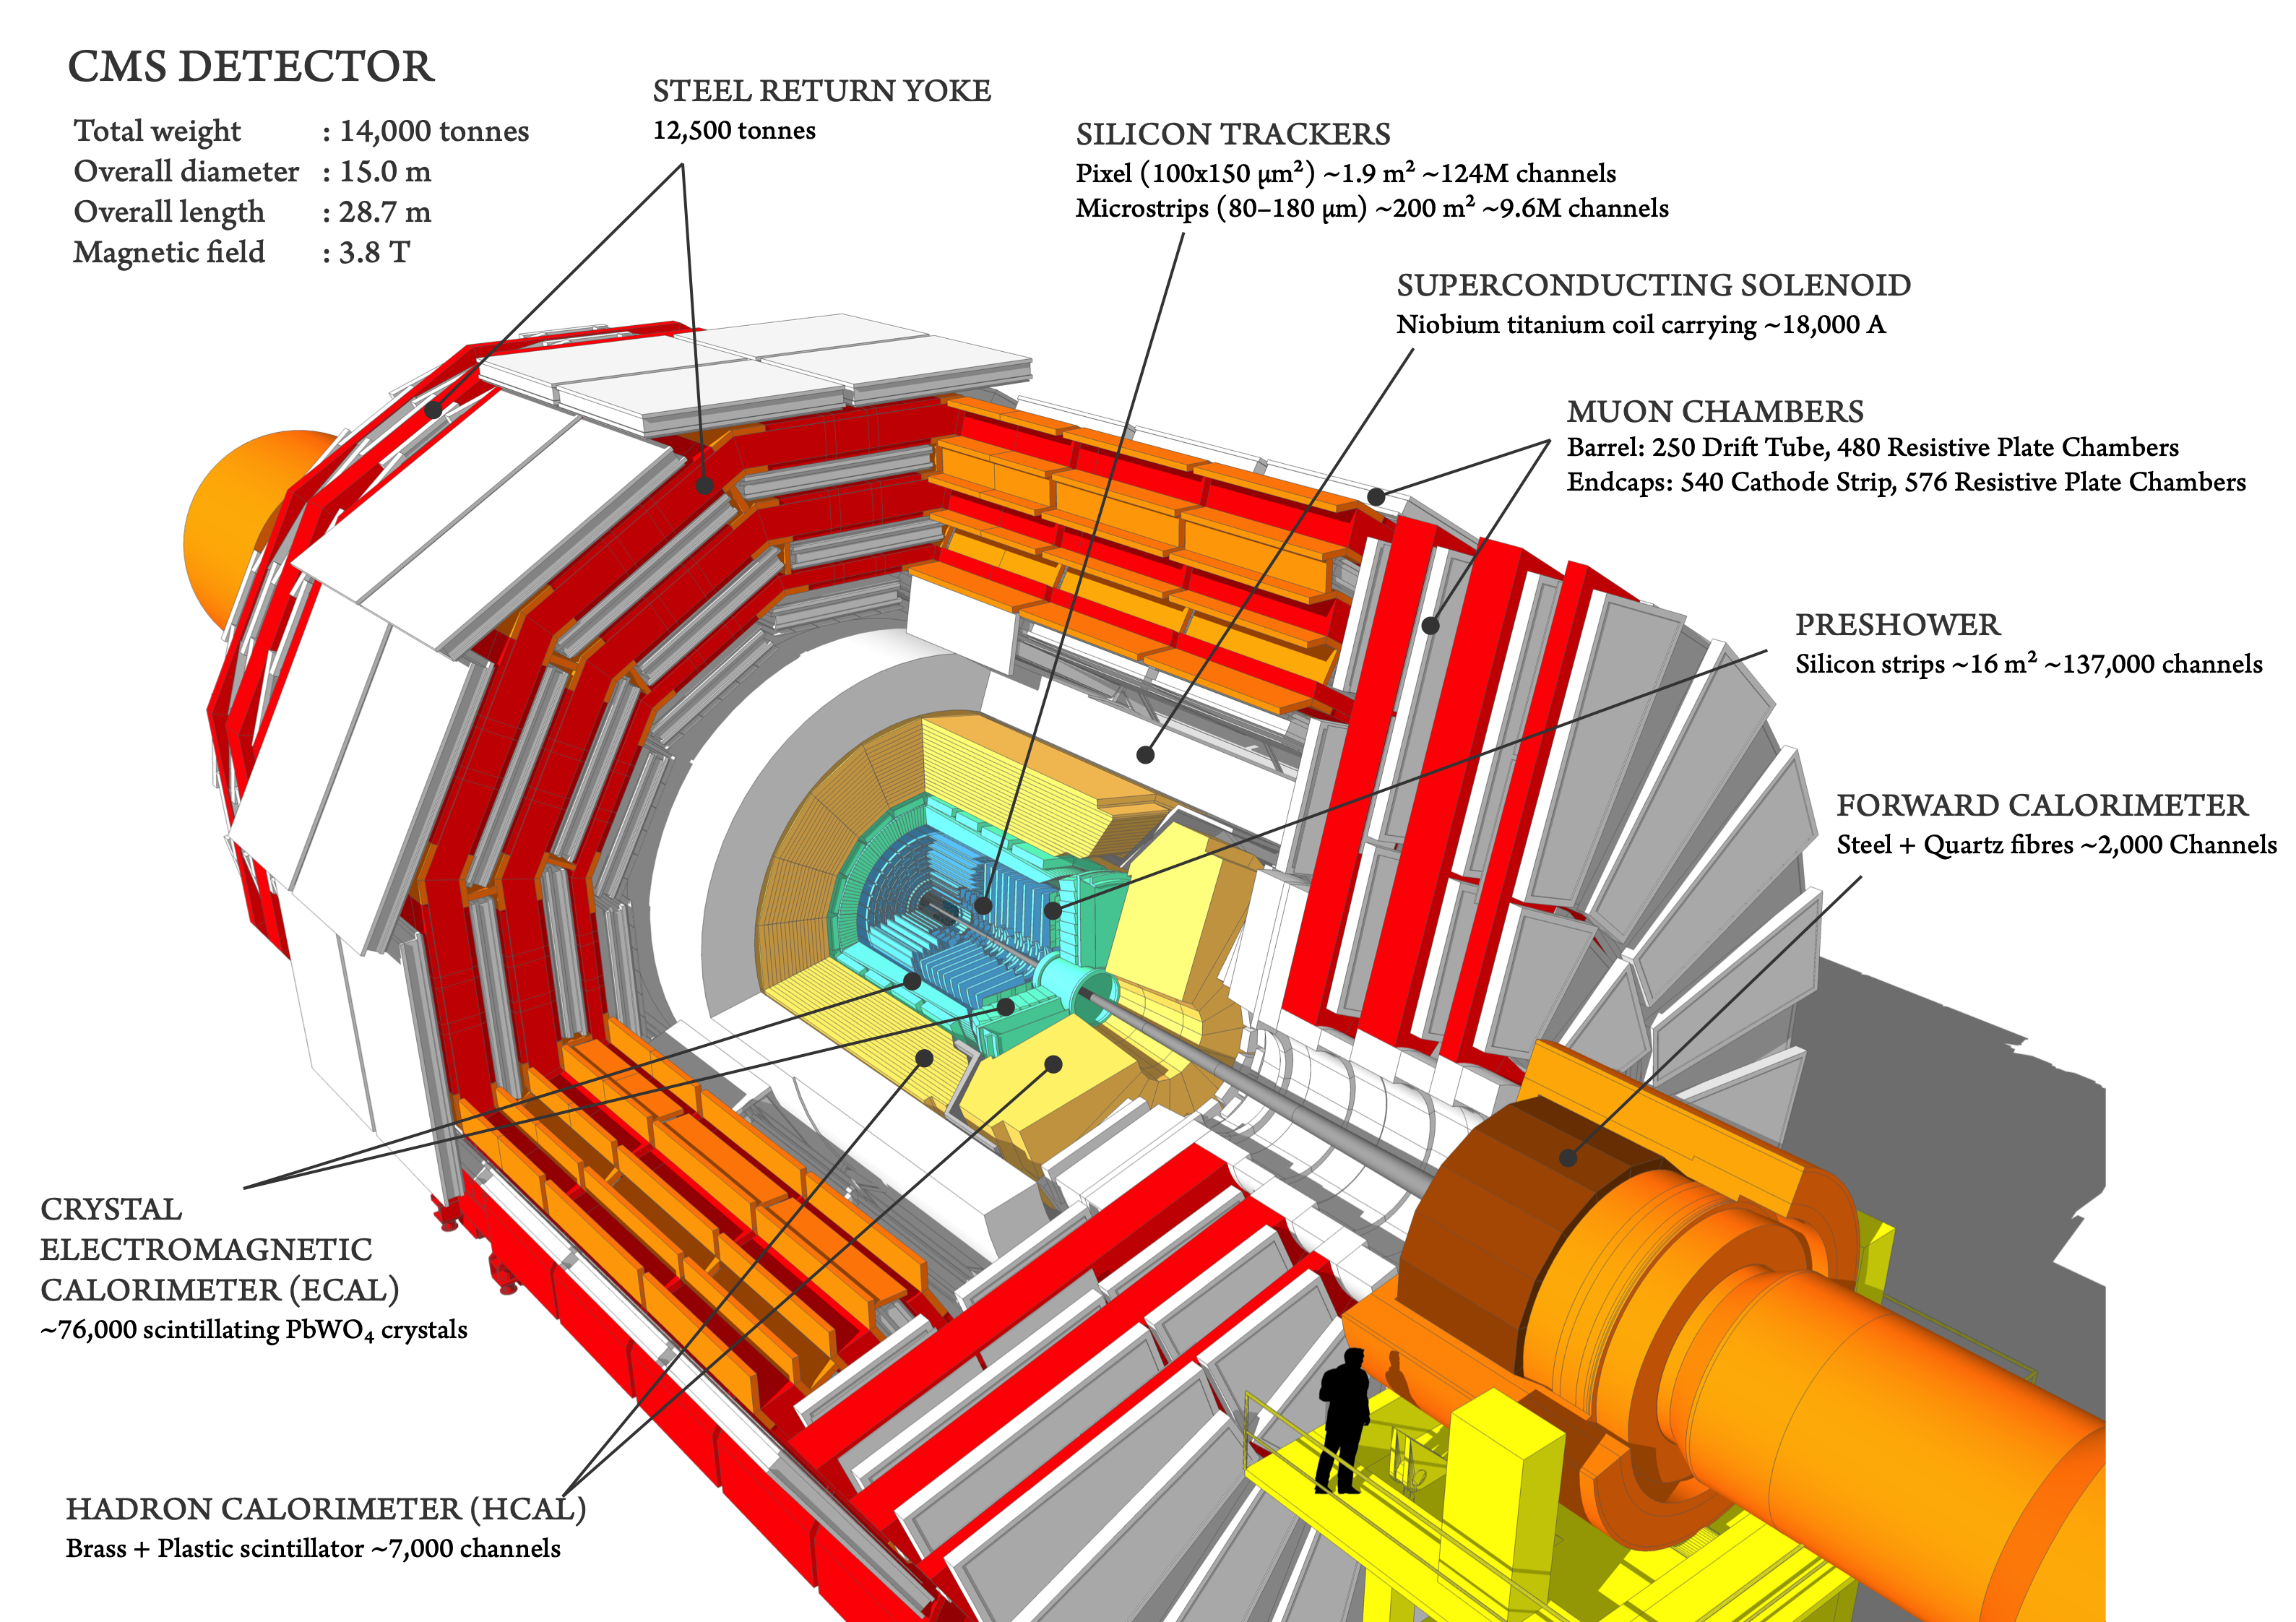
\includegraphics[width=0.75\paperwidth]{cms_160312_06b}}
%	\caption{Cutaway diagram of the CMS detector \cite{Sakuma_2014}}

%\end{figure}

%\begin{figure}
%\centerline{
%	\includegraphics[width=0.75\paperwidth]{CCC-v2019-final-white}}
%	\caption{CERN Accelerators complex \cite{Mobs:2684277}}
%\end{figure}







High Energy Phisics experiments need to collect a large quantity of data to attack the statistical nature of particle physics and find interesting phenomena with enough accuracy.

Many events searched by LHC require very rare and short-lived conditions:

ADD FIGURE

Statistical and random uncertainties follow known distributions (like a Poisson rate) or are empirically determined. Repeating measurements provides larger samples to estimate these uncertanties.


\section{Common Probability Distributions in Physics}

Many problems in physics are described or can be approximated by a small group of probability distributions \cite{leo2012techniques}.

\subsection{Binomial}
TODO
\subsection{Poisson}



\begin{equation}
	\label{eqn:poisson}
	P\left( x \right) = \frac{{e^{ - \lambda } \lambda ^x }}{{x!}}
\end{equation}

Consider the radioactive decay phenomena as an example: a radioactive source such as $^{137}$Cs has a half-life of 27 years. The probability for a single nucleus to decay is $8.2 \times 10^{-10}s^{-1}$. However, even a \SI{1}{\micro\gram} contains $10^{15}$ nuclei. Since each nucleus acts as a "trial", the mean number of decay events will be $\mu = N p$, satisfying the limiting conditions. The probability of observing an event is given by \ref{eqn:poisson}.

\subsection{Gaussian}

\section{CERN and the LHC}

\textit{luminosity} value of $10^{34}$ $cm^{-2}$ $s^{-1}$. This value is a measurement of the number of collisions that can be produced in a detector per $cm^2$ and per second.

\section{CMS}

\section{CMS Trigger System}


The LHC generates 40 milions events per second. Each CMS event, on average, carries a payload of 1 MB of unprocessed informations. It is technologically impossible to retain this amount of data, due to hardware, software, network and storage constraints.

Furthermore, most events represent uninteresting information for the current state of physics knowledge.

The \textit{CMS Trigger System} is designed to reduce the output stream to 1000 events per second, while preserving the physics reach of the experiment.
It is composed by a hierchical set of rules, called Trigger Nodes (or Paths): each one probes a specific patterns (physics signature) in the event or looks for specific physics objects.

This happens in two steps:

\begin{enumerate}

	\item The first level (L1) \cite{Bayatyan:706847} brings the 40 MHz to a 100 kHz rate. Here, N Trigger Algorithms are implemented on custom electronics (FPGAs and ASICs) exploiting informations from sub-detector components.

	\item A configurable set of L1 Trigger Nodes seeds Triggers in the second level (HLT), implemented in software. The event stream is further refined, selecting an average rate of 400 Hz for offline event storage and certification \cite{Khachatryan_2017}. HLT runs 600 of these independent Trigger Paths.

\end{enumerate}